\documentclass[11pt,aspectratio=169]{beamer}

\usetheme{Madrid}
\usecolortheme{default}
\setbeamertemplate{navigation symbols}{}
\setbeamertemplate{footline}{\hfill\usebeamercolor[fg]{structure}\small\insertframenumber/10\hspace{0.4cm}\vspace{0.15cm}}

\usepackage{booktabs,array}
\usepackage{graphicx}
\usepackage{tikz}
\usetikzlibrary{arrows.meta,positioning,calc}
\input{beamer_setup.tex}

% Optional fast part build; each p{n}-prefixed part overwrites
% tmp/<part-name>/preview.*.
\ifdefined\onlyframes
  \expandafter\includeonlyframes\expandafter{\onlyframes}
\fi

\definecolor{positive}{HTML}{0173B2}
\definecolor{negative}{HTML}{DE8F05}
\definecolor{emphasis}{HTML}{027A5A}
\definecolor{neutral}{HTML}{666666}
\definecolor{selPurple}{HTML}{7030A0}
\definecolor{selGreen}{HTML}{00A651}
\setbeamercolor{structure}{fg=positive}
\setbeamercolor{block title}{fg=white,bg=positive}
\setbeamercolor{block body}{fg=black,bg=positive!8}
\setbeamercolor{block title alerted}{fg=white,bg=negative}
\setbeamercolor{block body alerted}{fg=black,bg=negative!10}
\setbeamercolor{block title example}{fg=white,bg=emphasis}
\setbeamercolor{block body example}{fg=black,bg=emphasis!8}
\newcommand{\pos}[1]{\textcolor{positive}{#1}}
\newcommand{\con}[1]{\textcolor{negative}{#1}}
\newcommand{\HL}[1]{\textcolor{emphasis}{#1}}
\newcommand{\muted}[1]{\textcolor{neutral}{#1}}

\newcommand{\var}[1]{\texttt{\detokenize{#1}}}
\newcommand{\talkfig}[2][0.70\textheight]{\includegraphics[width=\linewidth,height=#1,keepaspectratio]{\csname source#2\endcsname}\par}
\newcommand{\draftline}{\par\vspace{0.35em}{\centering\small\color{neutral}\textit{DRAFT -- needs physics approval}\par}}
\newcommand{\notelead}[1]{\par{\color{positive}\bfseries #1}\par\vspace{0.25em}}
\newcommand{\caution}[1]{\par{\small\color{neutral}#1\par}}
\newcommand{\takeaway}[1]{\par\vspace{0.4em}{\small\color{positive}#1\par}}
\tikzset{box/.style={draw=positive,rounded corners=3pt,fill=positive!7,align=center,font=\small,inner sep=6pt},arr/.style={-{Stealth},thick,positive}}
\newcolumntype{L}[1]{>{\raggedright\arraybackslash}p{#1}}
\setlength{\tabcolsep}{5pt}
\renewcommand{\arraystretch}{1.18}
% Approved title for the 20260916 update.
\title[X(3872) Analysis Update]{X(3872) Analysis Update}
\author{\texorpdfstring{%
  Henrique Legoinha, \underline{Lekai Yao}, Nuno Leonardo,\\[0.15em]
  Yen-Jie Lee, Zhen Hu\\[0.45em]
  2026.9.16%
}{Henrique Legoinha, Lekai Yao, Nuno Leonardo, Yen-Jie Lee, Zhen Hu}}
\institute{}
\hypersetup{%
  pdfauthor={Henrique Legoinha, Lekai Yao, Nuno Leonardo, Yen-Jie Lee, Zhen Hu},
  pdftitle={X(3872) Analysis Update -- 2026.9.16},
  pdfsubject={Analysis update -- 2026.9.16}%
}
\date{%
  
\includegraphics[height=1.50cm]{figures/logos/CERN.png}\hspace{0.25cm}%
  
\includegraphics[height=1.50cm]{figures/logos/CMS.png}\hspace{0.25cm}%
  
\includegraphics[height=1.50cm]{figures/logos/LIP.png}\hspace{0.25cm}%
  
\includegraphics[height=1.50cm]{figures/logos/IST.png}\hspace{0.25cm}%
  
\includegraphics[height=1.50cm]{figures/logos/THU.png}\hspace{0.25cm}%
  
\includegraphics[height=1.50cm]{figures/logos/MIT.png}%
}

\pdfstringdefDisableCommands{\def\translate#1{#1}}

\begin{document}

% P1--P13 approved by the user on 20260916; P11--P13 are backup.
\begin{frame}[plain,label=p1_20260916]
  \titlepage
\end{frame}

% 20260916 user-directed recap. rw means reweighting, not MC generation weights.
% Historical context: docs/slides_terminology.md and the archived workflow.
% Current inputs: accepted H045/H046 intake; no new validation claim.
\begin{frame}[label=p2_20260916]{Recap: from reweighting to direct ML selection}
  \begin{center}
  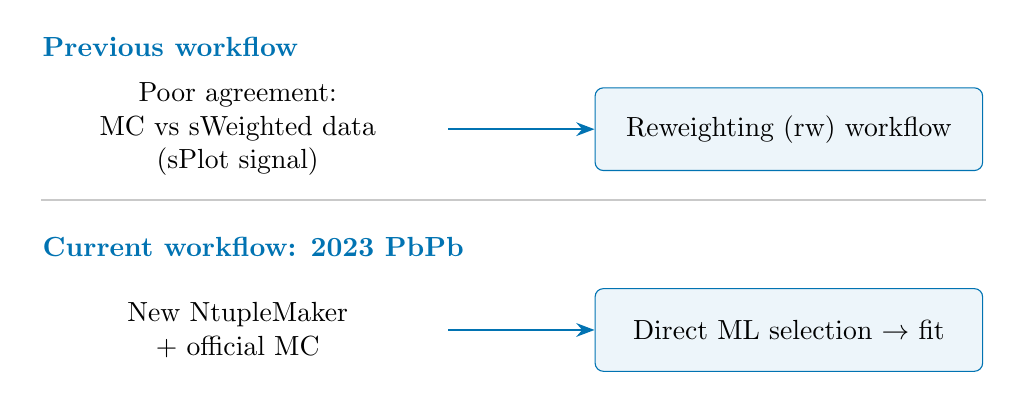
\begin{tikzpicture}
    \node[anchor=west,text=positive,font=\bfseries] at (-6.1,1.5) {Previous workflow};
    \node[align=center,text width=5.1cm] (old) at (-3.5,0.45)
      {Poor agreement:\\MC vs sWeighted data\\(sPlot signal)};
    \node[box,text width=4.5cm,font=\normalsize,minimum height=1.05cm] (rw) at (3.5,0.45)
      {Reweighting (rw) workflow};
    \draw[arr] (old.east)--(rw.west);
    \draw[neutral!35] (-6.0,-0.45)--(6.0,-0.45);
    \node[anchor=west,text=positive,font=\bfseries] at (-6.1,-1.05) {Current workflow: 2023 PbPb};
    \node[align=center,text width=5.1cm] (now) at (-3.5,-2.1)
      {New NtupleMaker\\+ official MC};
    \node[box,text width=4.5cm,font=\normalsize,minimum height=1.05cm] (ml) at (3.5,-2.1)
      {Direct ML selection $\rightarrow$ fit};
    \draw[arr] (now.east)--(ml.west);
  \end{tikzpicture}
  \end{center}
\end{frame}

% Five configurations: accepted H045 nodes.csv; names allowed by user.
\begin{frame}[label=p3_20260916]{Five ML configurations: inputs and selections}
  \relax
  {\small
  \textbf{Common inputs:} \var{Bmu1pt}, \var{Bmu1eta}, \var{Bmu2pt}, \var{Bmu2eta}, \var{Btrk2Pt}, \var{BtrkPtimb}.\par\vspace{0.3em}
  \textbf{Common selection:} \var{Bpt}$<50$ GeV, $|\var{By}|<1.6$, \var{BQvalue}$<0.15$ GeV.
  }
  \begin{center}\small
  \setlength{\tabcolsep}{3pt}\renewcommand{\arraystretch}{1.00}
  \begin{tabular}{@{}L{1.10cm}L{3.50cm}L{1.30cm}L{1.75cm}L{1.75cm}L{2.25cm}@{}}
    \toprule
    Config. & Additional inputs & \var{Bpt} (GeV) & \var{Btrk1dR} & \var{Btrk2dR} & Sidebands (GeV)\\
    \midrule
    1 & \var{Bmu1phi}, \var{Bmu2phi}, \var{Btrk1dR} & $>10$ & No cut & $(0,0.25)$ & (3.82,3.85); (3.89,3.92)\\
    2 & \var{Bmu1phi}, \var{Bmu2phi} & $>10$ & $(0,0.25)$ & $(0,0.25)$ & (3.75,3.85); (3.90,4.00)\\
    3 & \var{Btrk1dR}, \var{Bujeta}, \var{Btktketa} & $>10$ & No cut & $(0,0.25)$ & (3.82,3.85); (3.89,3.92)\\
    4 & Same as 3 & $>15$ & No cut & $(0,0.25)$ & (3.82,3.85); (3.89,3.92)\\
    5 & Same as 3 & $>15$ & No cut & $(0,0.35)$ & (3.80,3.85); (3.89,3.94)\\
    \bottomrule
  \end{tabular}
  \end{center}
  \caution{Sidebands define the training background; intervals have strict bounds.}
\end{frame}

\begin{frame}[label=p4_20260916]{Configuration 1: selected mass spectrum and fit}
  \relax
  {\small Relative weighted X-MC efficiency: 25\%; score $>0.95279$.}\par
  \begin{columns}[T]
    \column{0.48\textwidth}\centering
    {\small\textbf{cut\_scan: selected DATA}}\par
    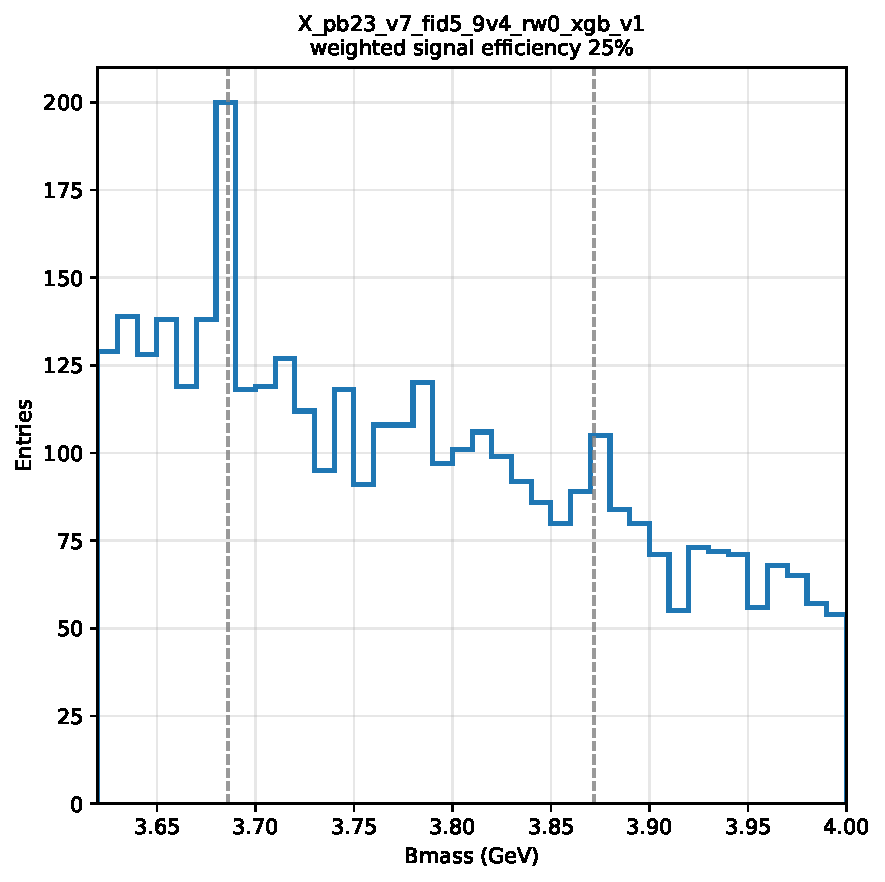
\includegraphics[width=\linewidth,height=0.52\textheight,keepaspectratio]{figures/20260916/config1_cut_scan.pdf}
    \column{0.48\textwidth}\centering
    {\small\textbf{Default single-X fit}}\par
    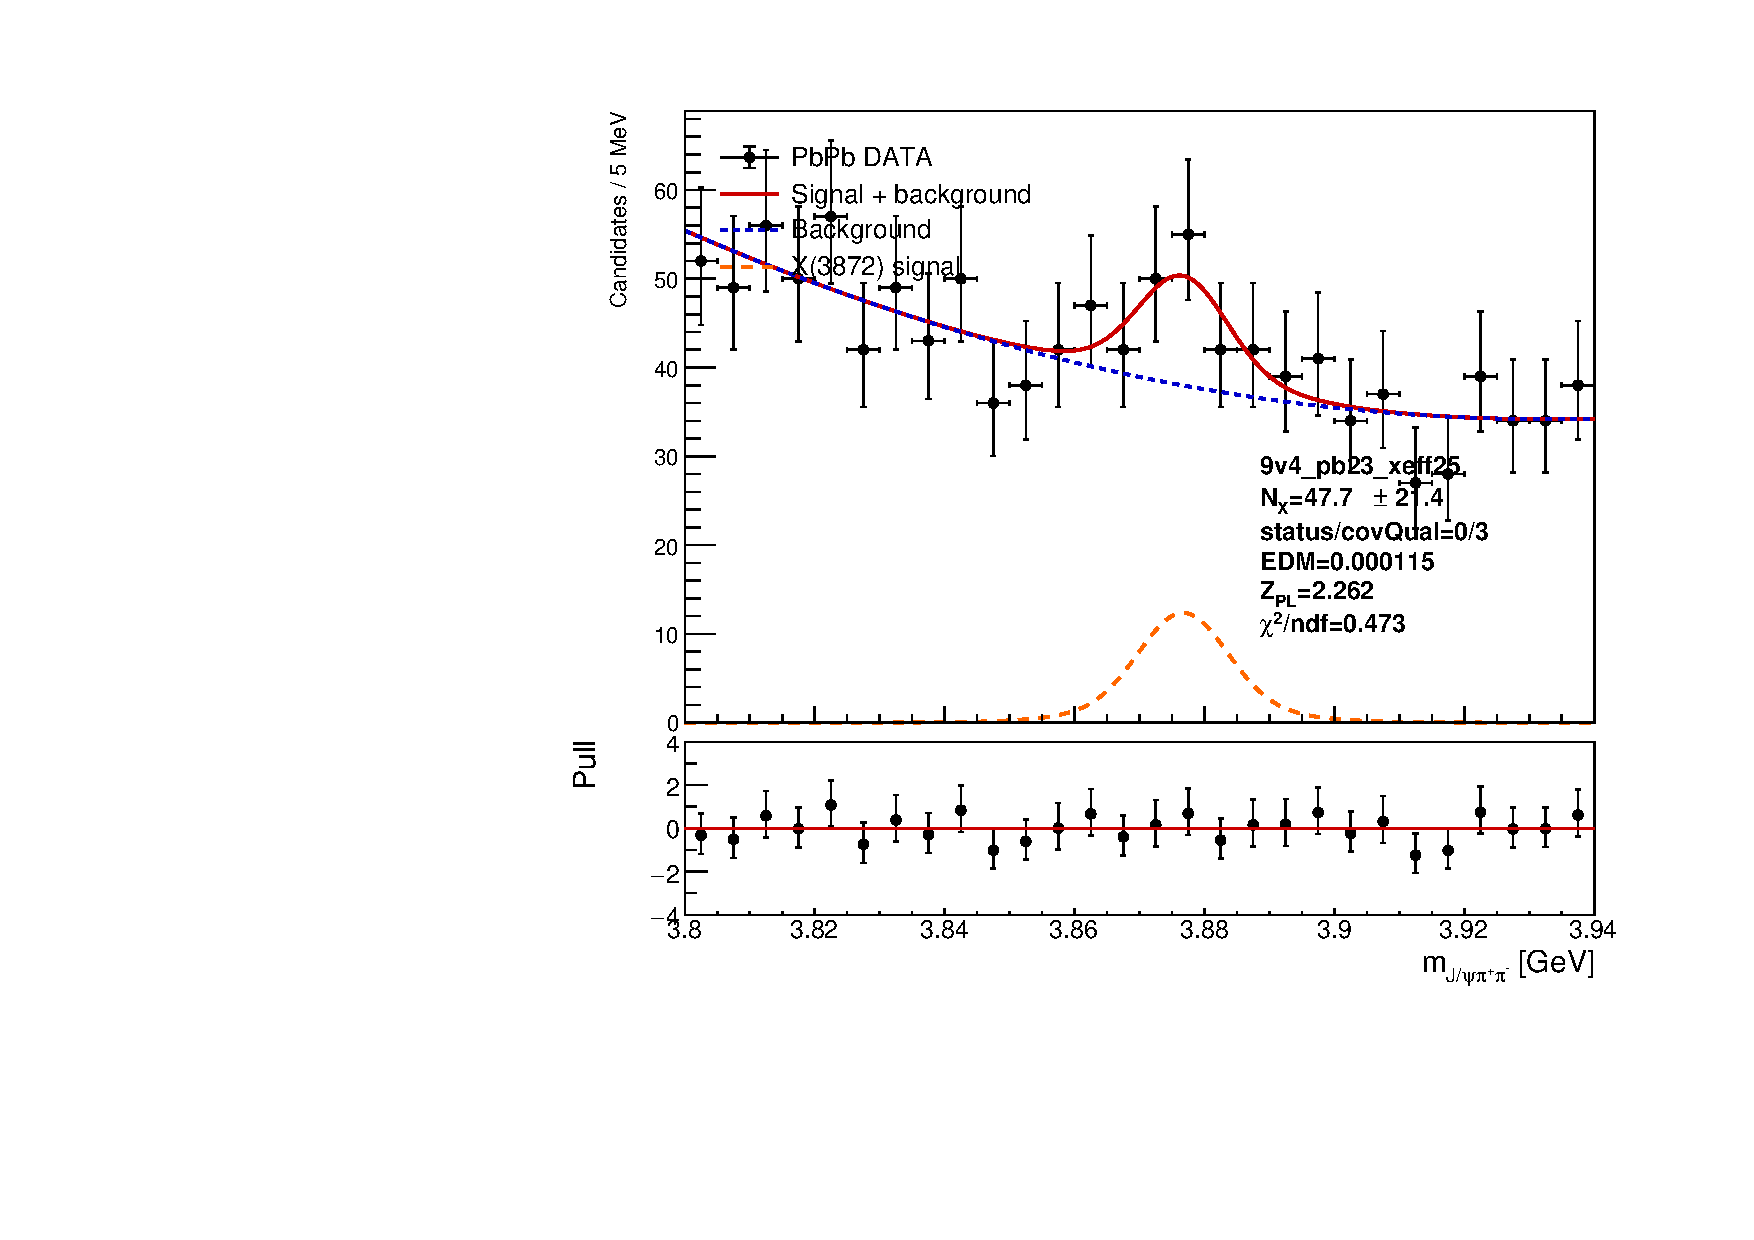
\includegraphics[width=\linewidth,height=0.52\textheight,keepaspectratio]{figures/20260916/config1_fit.pdf}
  \end{columns}
  {\small $N_X=47.71\pm21.44$;\quad $\mu_X=3876.69\pm7.51$ MeV;\quad scale $=1.500$.}\par
  {\small Significance: $2.262$.}\par
  \caution{Mean and scale at their upper bounds. Fit range: 3.80--3.94 GeV.}
\end{frame}

\begin{frame}[label=p5_20260916]{Configuration 2: selected mass spectrum and fit}
  \relax
  {\small Relative weighted X-MC efficiency: 40\%; score $>0.86855$.}\par
  \begin{columns}[T]
    \column{0.48\textwidth}\centering
    {\small\textbf{cut\_scan: selected DATA}}\par
    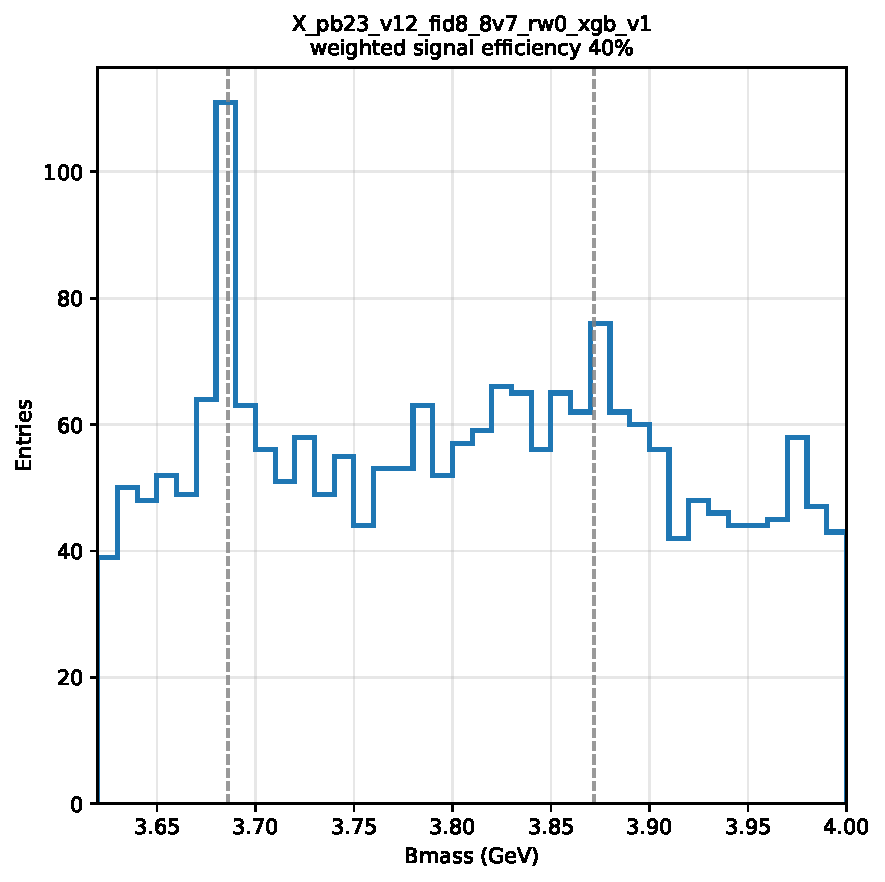
\includegraphics[width=\linewidth,height=0.52\textheight,keepaspectratio]{figures/20260916/config2_cut_scan.pdf}
    \column{0.48\textwidth}\centering
    {\small\textbf{Default single-X fit}}\par
    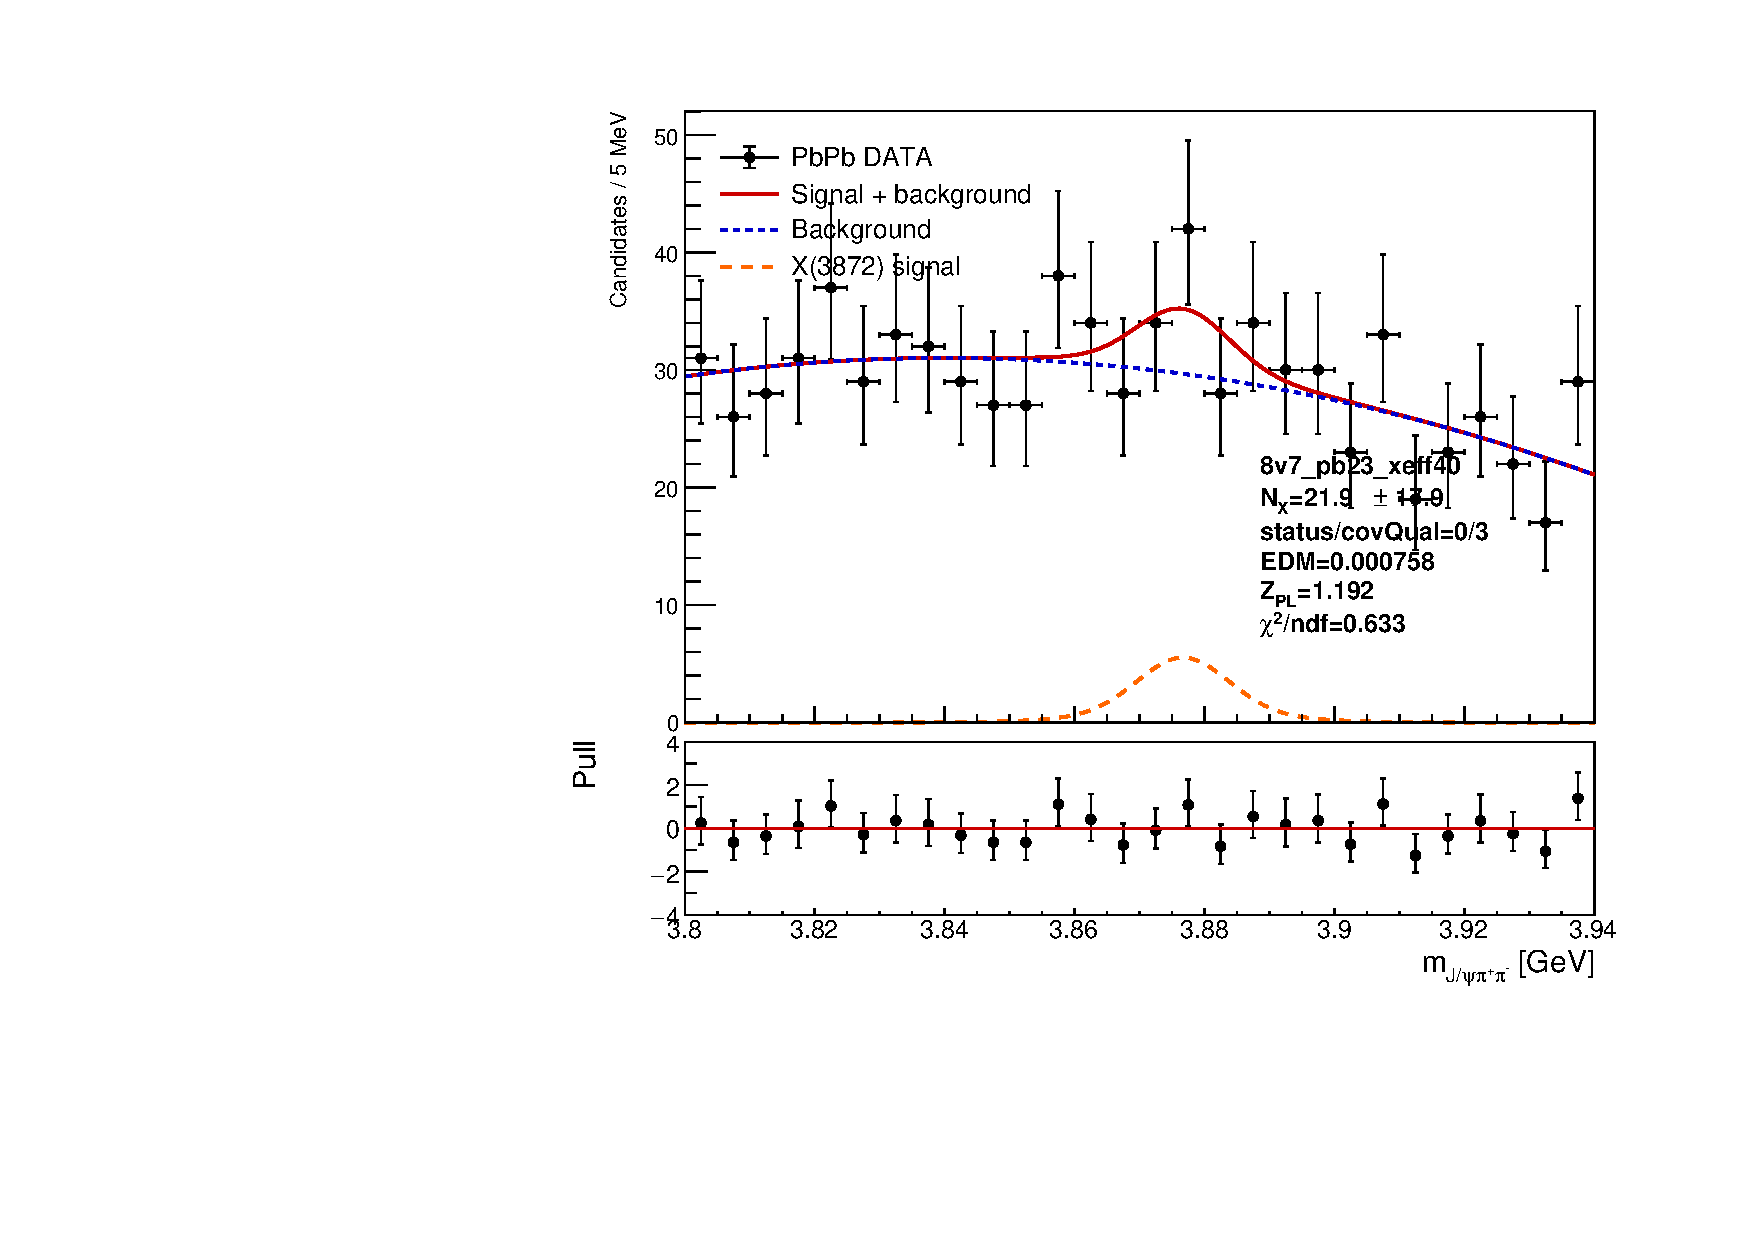
\includegraphics[width=\linewidth,height=0.52\textheight,keepaspectratio]{figures/20260916/config2_fit.pdf}
  \end{columns}
  {\small $N_X=21.94\pm17.92$;\quad $\mu_X=3876.69\pm6.90$ MeV;\quad scale $=1.500$.}\par
  {\small Significance: $1.192$.}\par
  \caution{Mean and scale at their upper bounds. Fit range: 3.80--3.94 GeV.}
\end{frame}

\begin{frame}[label=p6_20260916]{Configuration 3: selected mass spectrum and fit}
  \relax
  {\small Relative weighted X-MC efficiency: 25\%; score $>0.95267$.}\par
  \begin{columns}[T]
    \column{0.48\textwidth}\centering
    {\small\textbf{cut\_scan: selected DATA}}\par
    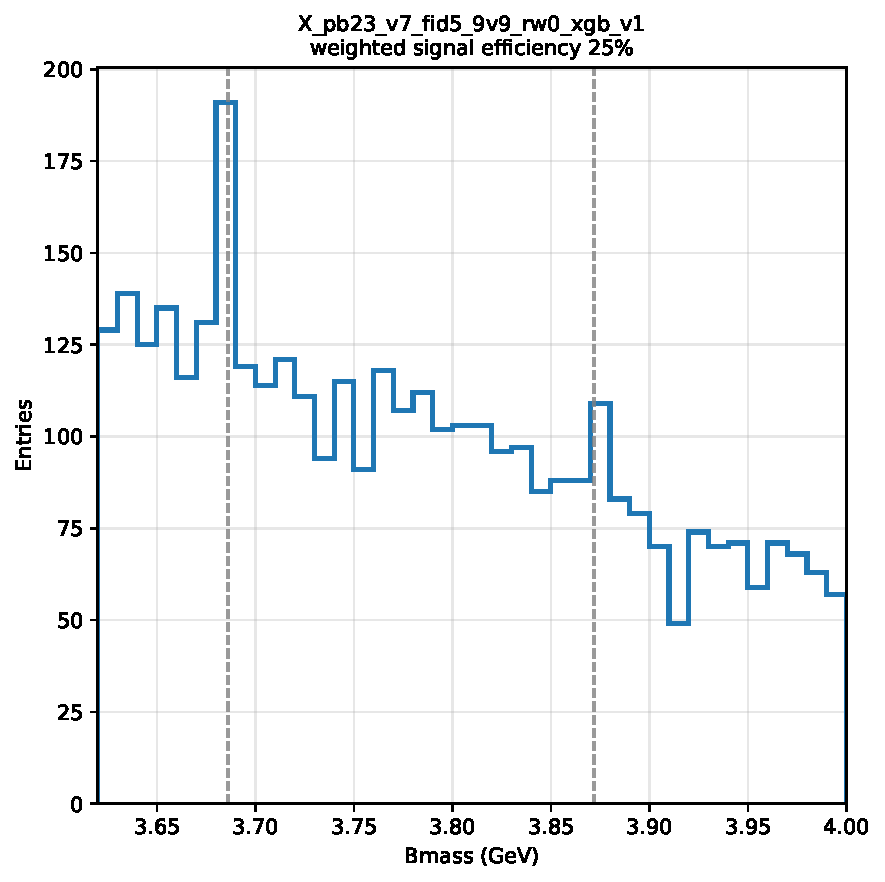
\includegraphics[width=\linewidth,height=0.52\textheight,keepaspectratio]{figures/20260916/config3_cut_scan.pdf}
    \column{0.48\textwidth}\centering
    {\small\textbf{Default single-X fit}}\par
    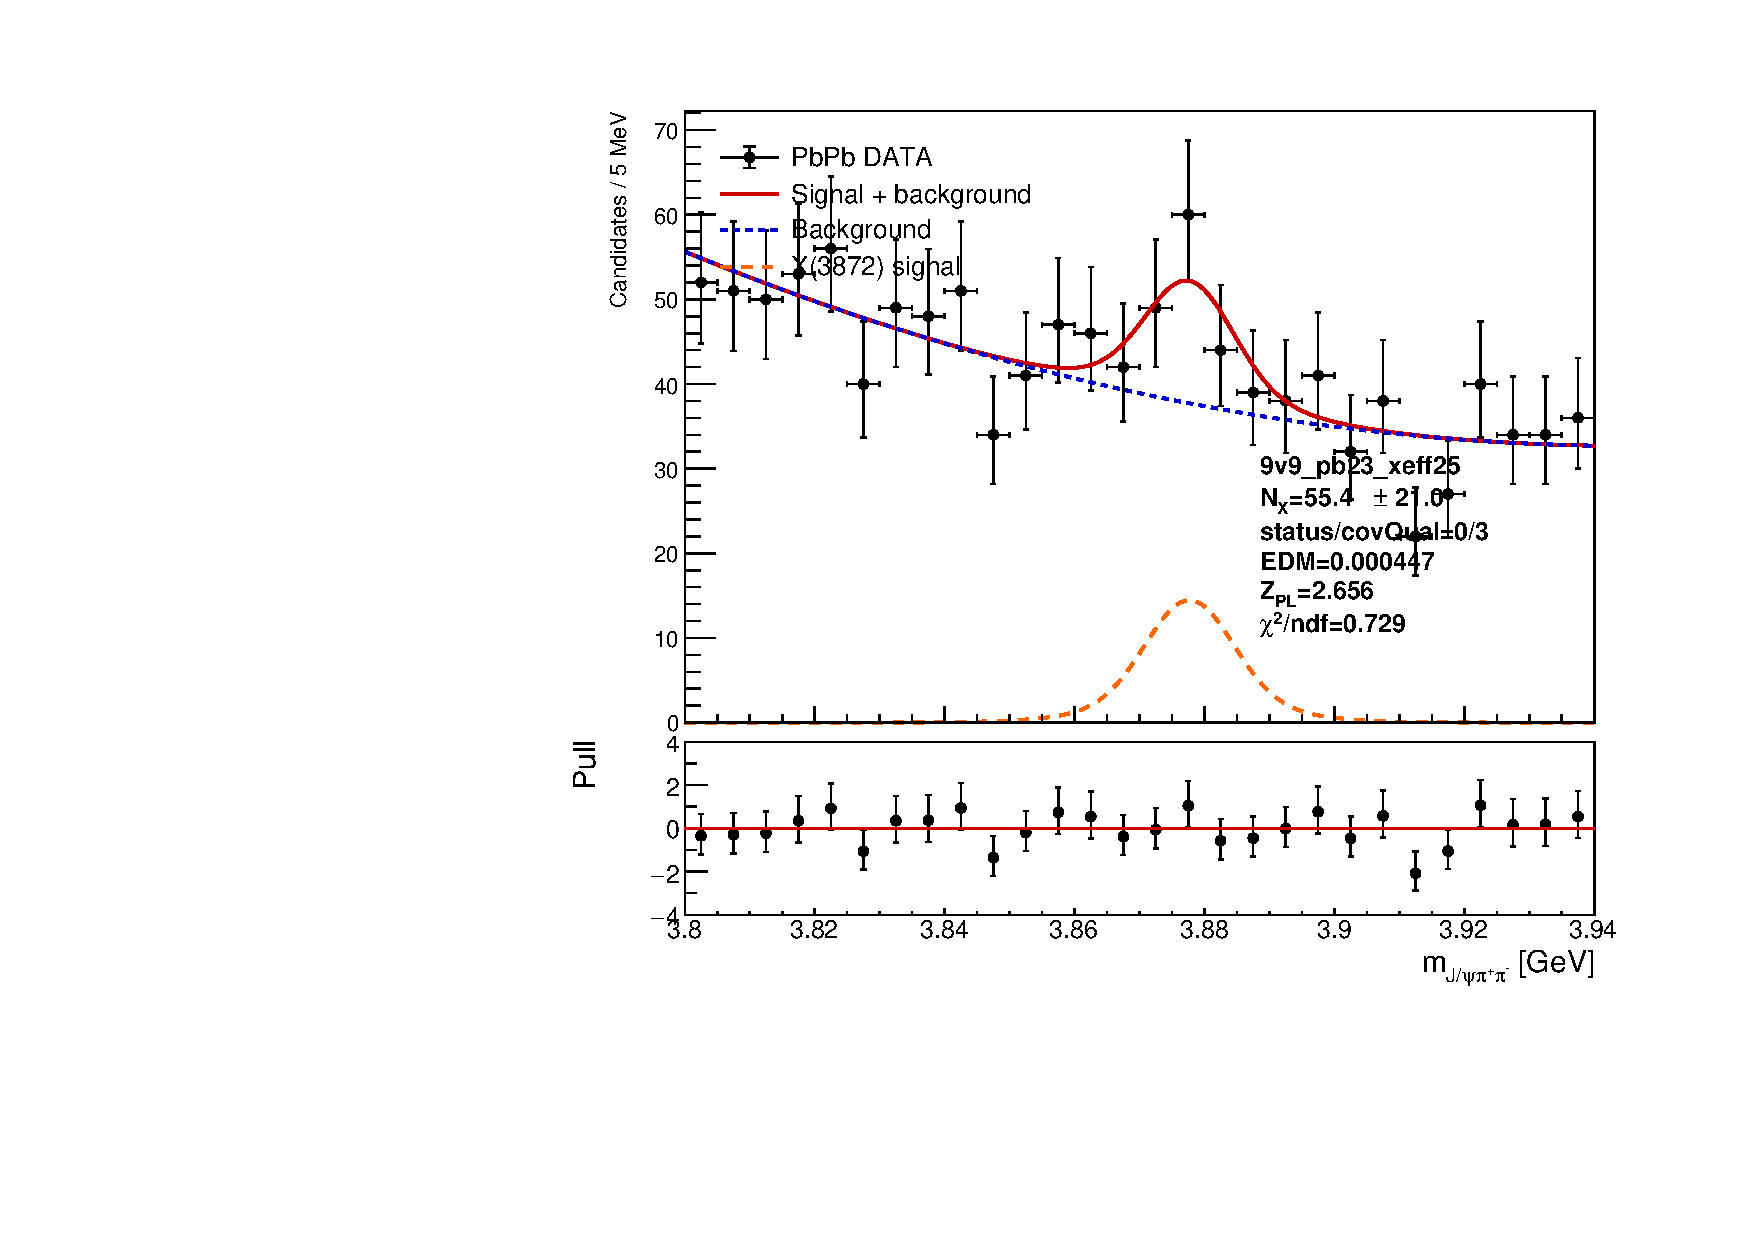
\includegraphics[width=\linewidth,height=0.52\textheight,keepaspectratio]{figures/20260916/config3_fit.pdf}
  \end{columns}
  {\small $N_X=55.42\pm21.04$;\quad $\mu_X=3877.67\pm2.82$ MeV;\quad scale $=1.495$.}\par
  {\small Significance: $2.656$.}\par
  \caution{Mean range: nominal $\pm10$ MeV; scale range: [0.5,1.5]. Fit range: 3.80--3.94 GeV.}
\end{frame}

\begin{frame}[label=p7_20260916]{Configuration 4: selected mass spectrum and fit}
  \relax
  {\small Relative weighted X-MC efficiency: 40\%; score $>0.84505$.}\par
  \begin{columns}[T]
    \column{0.48\textwidth}\centering
    {\small\textbf{cut\_scan: selected DATA}}\par
    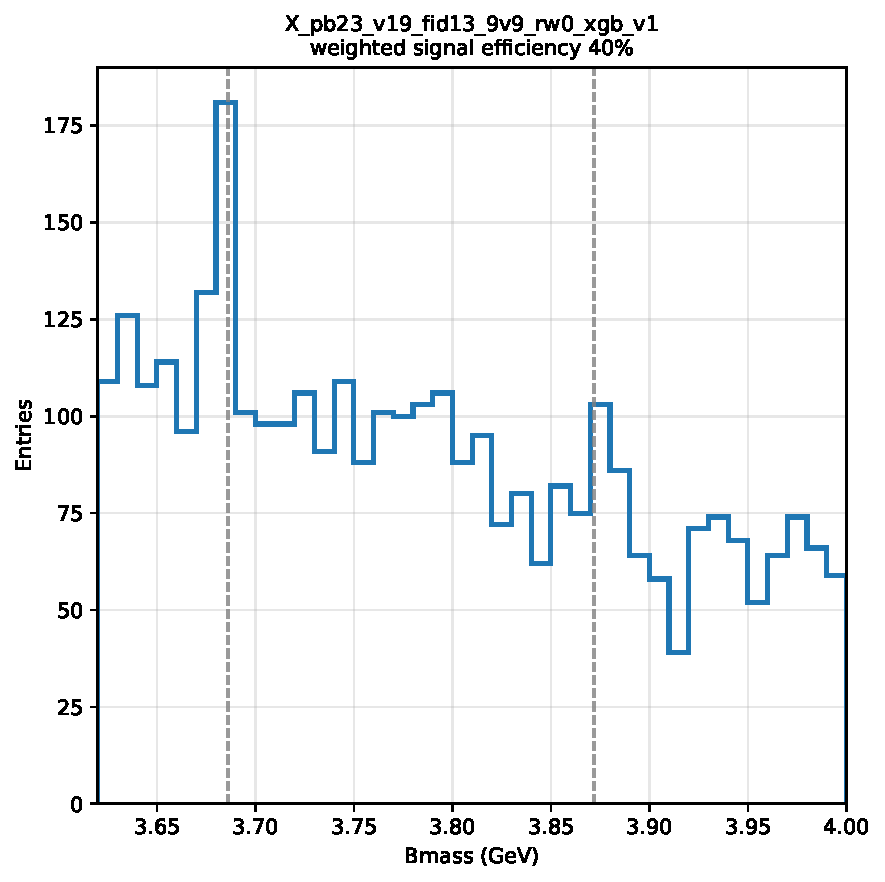
\includegraphics[width=\linewidth,height=0.52\textheight,keepaspectratio]{figures/20260916/config4_cut_scan.pdf}
    \column{0.48\textwidth}\centering
    {\small\textbf{Two-peak fit}}\par
    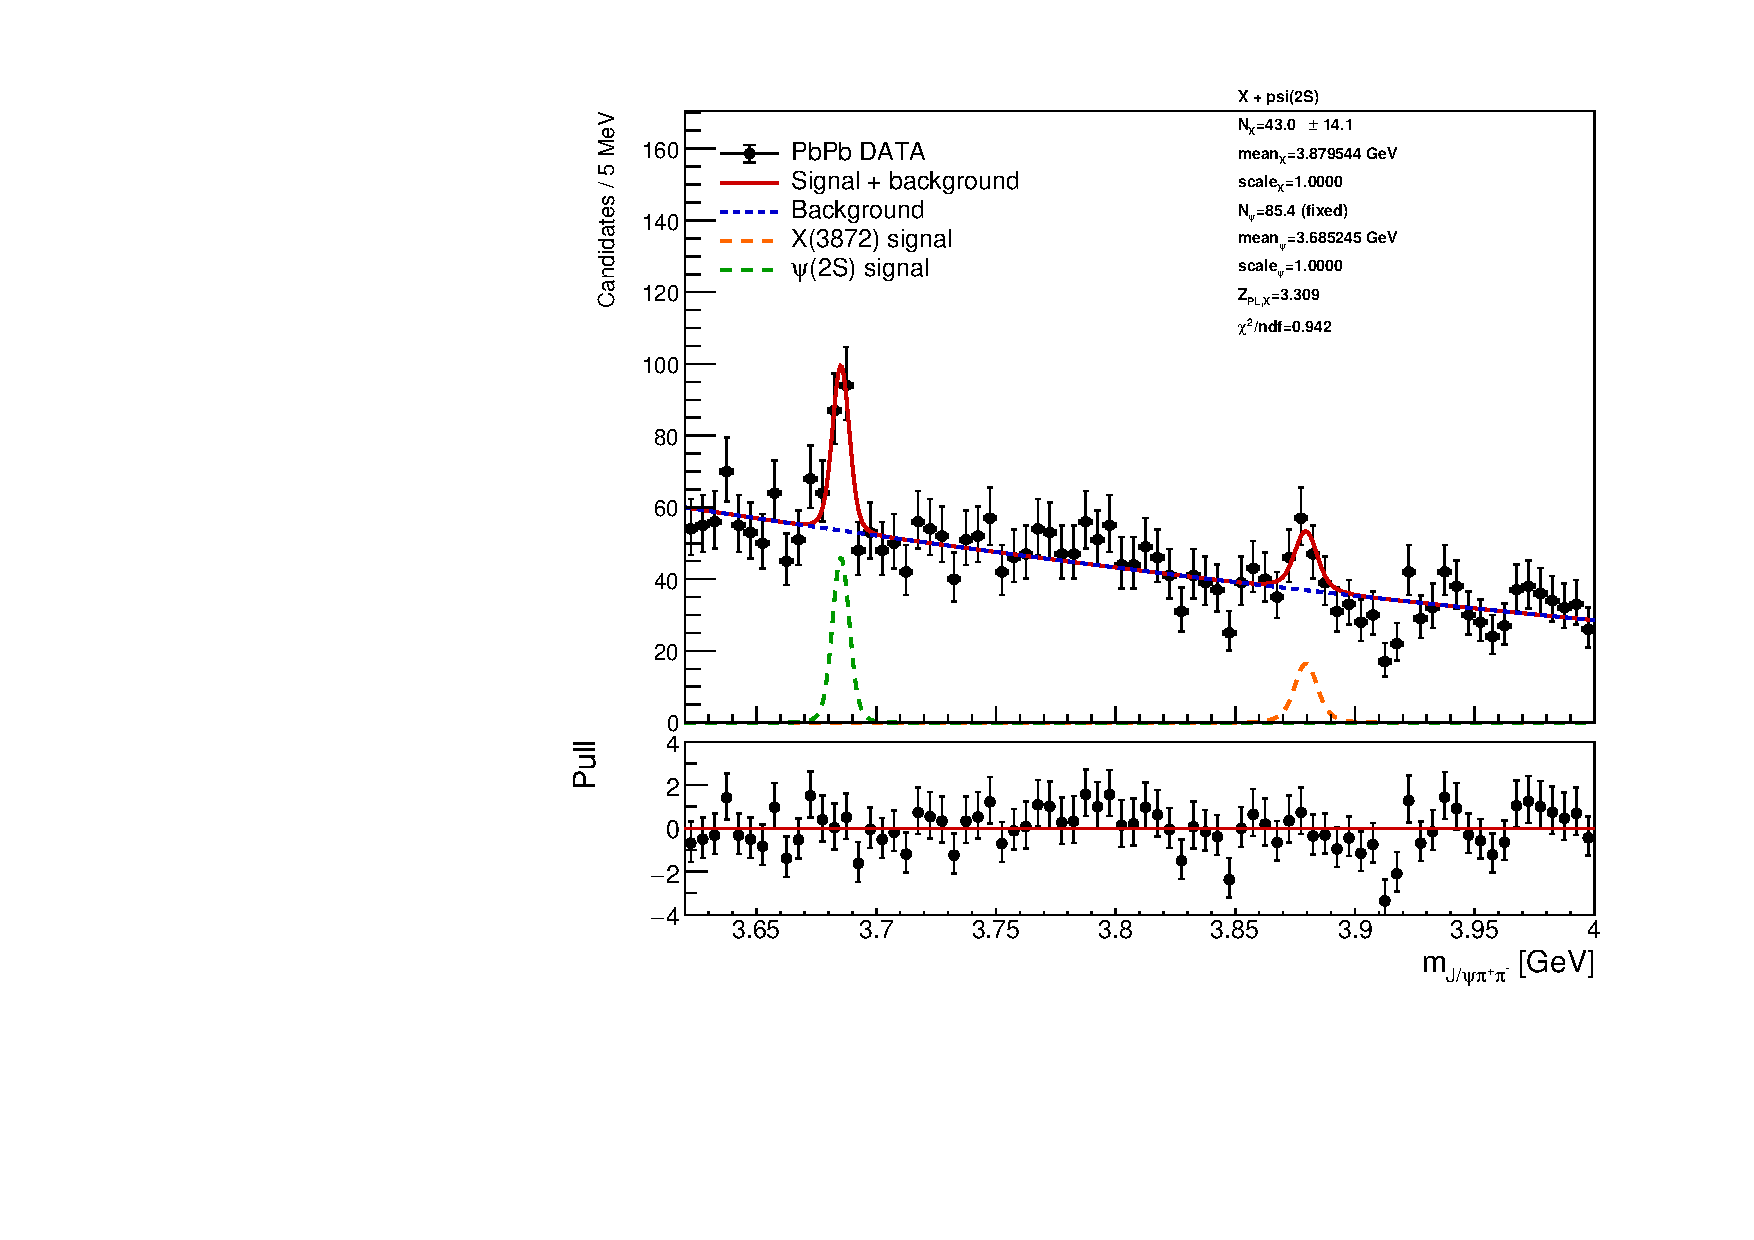
\includegraphics[width=\linewidth,height=0.52\textheight,keepaspectratio]{figures/20260916/config4_fit.pdf}
  \end{columns}
  {\small $N_X=42.98\pm14.11$;\quad $\mu_X=3879.54$ MeV.}\par
  {\small $N_\psi=85.41$;\quad $\mu_\psi=3685.24$ MeV.}\par
  {\small Significance: $3.309$.}\par
  \caution{Means and $N_\psi$ fixed from the first fit; both scales fixed to 1.}
\end{frame}

\begin{frame}[label=p8_20260916]{Configuration 5: selected mass spectrum and fit}
  \relax
  {\small Relative weighted X-MC efficiency: 50\%; score $>0.78272$.}\par
  \begin{columns}[T]
    \column{0.48\textwidth}\centering
    {\small\textbf{cut\_scan: selected DATA}}\par
    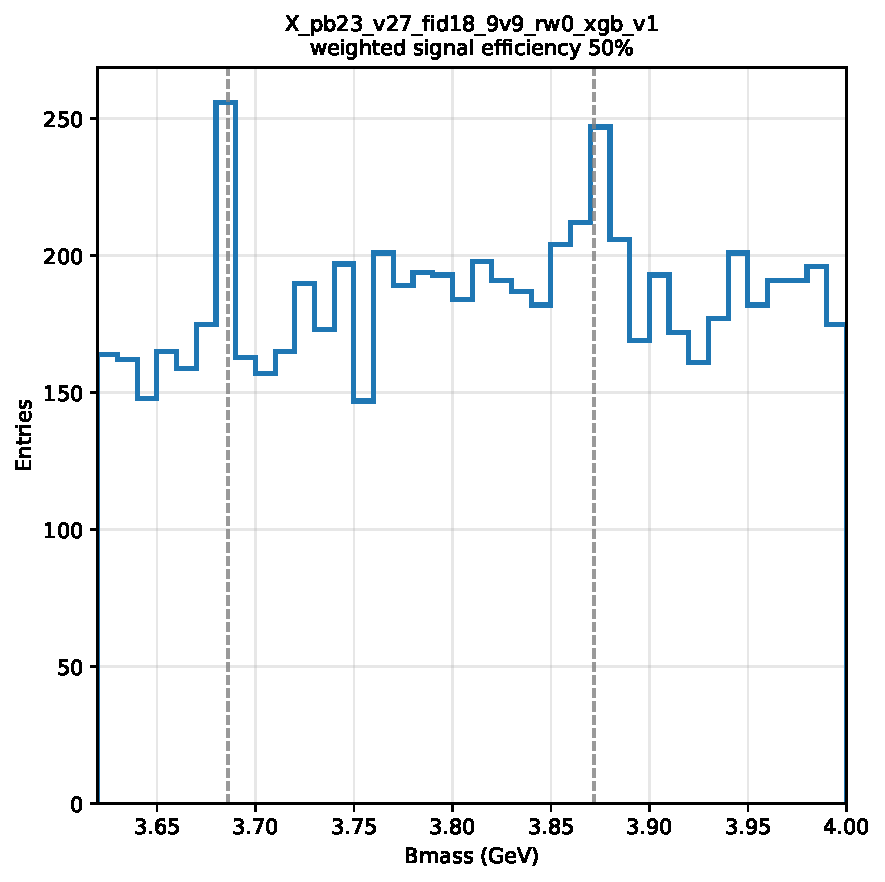
\includegraphics[width=\linewidth,height=0.52\textheight,keepaspectratio]{figures/20260916/config5_cut_scan.pdf}
    \column{0.48\textwidth}\centering
    {\small\textbf{Two-peak fit}}\par
    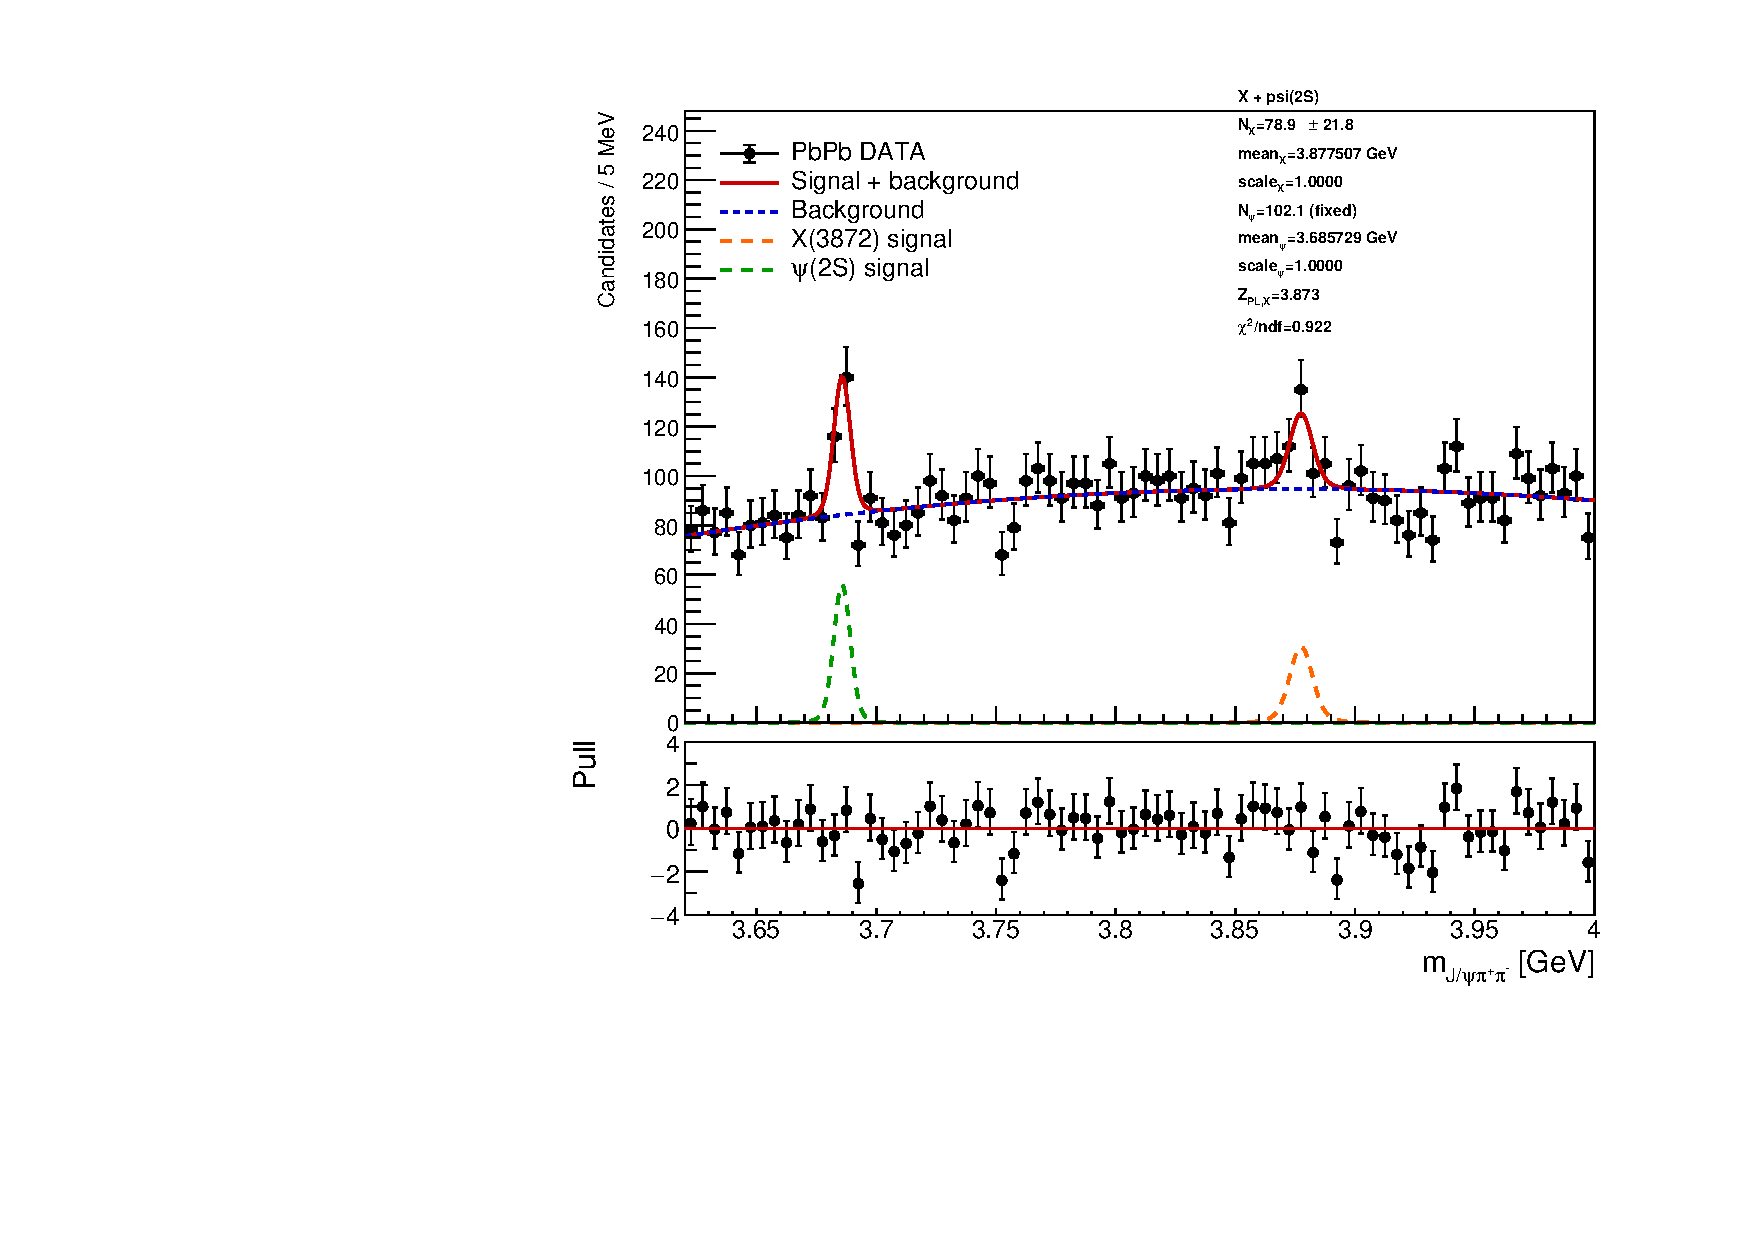
\includegraphics[width=\linewidth,height=0.52\textheight,keepaspectratio]{figures/20260916/config5_fit.pdf}
  \end{columns}
  {\small $N_X=78.88\pm21.76$;\quad $\mu_X=3877.51$ MeV.}\par
  {\small $N_\psi=102.07$;\quad $\mu_\psi=3685.73$ MeV.}\par
  {\small Significance: $3.873$.}\par
  \caution{Means and $N_\psi$ fixed from the first fit; both scales fixed to 1.}
\end{frame}

\begin{frame}[label=p9_20260916]{ML recipe comparison: summary}
  \begin{center}\small
  \renewcommand{\arraystretch}{1.15}
  \begin{tabular}{@{}cL{5.3cm}ccL{2.3cm}@{}}
    \toprule
    Config. & Main change & $\epsilon_X$ & $N_X$ & Significance\\
    \midrule
    1 & Nine-input starting point & 25\% & $47.7\pm21.4$ & 2.262\\
    2 & \var{Btrk1dR}: input $\to$ selection; wider sidebands & 40\% & $21.9\pm17.9$ & 1.192\\
    3 & Two muon $\phi$ inputs $\to$ \var{Bujeta}, \var{Btktketa} & 25\% & $55.4\pm21.0$ & 2.656\\
    4 & \var{Bpt}$>15$ GeV & 40\% & $43.0\pm14.1$ & 3.309\\
    5 & Wider \var{Btrk2dR} selection and sidebands & 50\% & $78.9\pm21.8$ & 3.873\\
    \bottomrule
  \end{tabular}
  \end{center}
  {\small\textbf{Tested alternatives with worse results:}}\par
  \begin{itemize}\small
    \item The configuration used in the previous analysis.
    \item Using both \var{Btrk1dR} and \var{Btrk2dR} as training inputs.
    \item Other previously useful variables: \var{Btktkpt}, \var{Balpha},
          \var{Bcos_dtheta}, \var{Bchi2Prob}.
  \end{itemize}
\end{frame}

\begin{frame}[label=p10_20260916]{\strut}
  \centering\vfill
  \makebox[\textwidth][c]{%
    \begin{beamercolorbox}[wd=0.68\textwidth,sep=1.2em,center,rounded=true,shadow=true]{block body}
      {\LARGE\bfseries Thanks for listening!}\par
      \vspace{1.0em}
      {\large Reporter: Lekai Yao}\par
      \vspace{0.45em}
      {\large 2026.9.16}
    \end{beamercolorbox}%
  }
  \vfill
\end{frame}


% Approved backup; retain the main-talk denominator of 10.
\appendix
\setbeamertemplate{footline}{\hfill\usebeamercolor[fg]{structure}\small Backup\quad\insertframenumber\hspace{0.4cm}\vspace{0.15cm}}
\begin{frame}[label=p11_20260916]{Backup: configuration 5 --- FOM definition}
  \relax
  {\small 2023 PbPb; configuration 5 selection. Scan $\epsilon_X=15$--$60\%$ in $1\%$ steps (46 points).}\par
  \vspace{0.15em}
  {\centering
  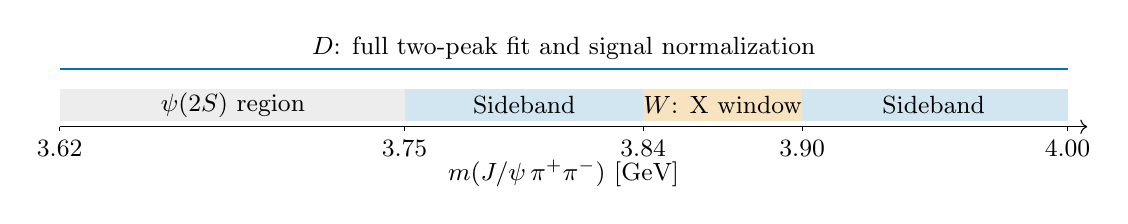
\begin{tikzpicture}[x=1cm,y=0.7cm,font=\small]
    \draw[positive,thick] (0,1.05)--(12.8,1.05);
    \node[above] at (6.4,1.05) {$D$: full two-peak fit and signal normalization};
    \fill[neutral!12] (0,0.10) rectangle (4.38,0.68);
    \fill[positive!18] (4.38,0.10) rectangle (7.41,0.68);
    \fill[negative!25] (7.41,0.10) rectangle (9.43,0.68);
    \fill[positive!18] (9.43,0.10) rectangle (12.8,0.68);
    \node at (2.2,0.39) {$\psi(2S)$ region};
    \node at (5.90,0.39) {Sideband};
    \node at (8.42,0.39) {$W$: X window};
    \node at (11.1,0.39) {Sideband};
    \draw[->] (0,0)--(13.05,0);
    \foreach \x/\mass in {0/3.62,4.38/3.75,7.41/3.84,9.43/3.90,12.8/4.00}{
      \draw (\x,0)--(\x,-0.08);\node[below] at (\x,-0.08) {\mass};}
    \node[below] at (6.4,-0.42) {$m(J/\psi\,\pi^+\pi^-)$ [GeV]};
  \end{tikzpicture}
  \par}
  \vspace{0.2em}
  {\small
  \textbf{Reference: 50\% efficiency}, score $>0.782725$; use one existing two-peak fit to normalize all cuts.\par
  $N_{\rm ref}=78.79\pm22.14$, $\mu_X=3877.51$ MeV: first fit with floating means and fixed MC widths.\par
  }
  \vspace{0.4em}
  \begin{columns}[T]
    \column{0.36\textwidth}\small
    \textbf{Expected signal in $W$}
    \[
      S_W(c)=N_{\rm ref}\frac{\epsilon_D(c)}{\epsilon_D(c_0)}A_W(c).
    \]
    \column{0.60\textwidth}\small
    $\epsilon_D$: \var{pThatreweight}-weighted MC efficiency in $D$.\par
    $A_W$: MC double-Gaussian integral ratio $W/D$;\par
    same-cut widths, fixed reference DATA mean and scale 1.
  \end{columns}
  \vspace{0.3em}
  {\small\textbf{Background in $W$:} unbinned second-order Chebyshev (C2) fit to\par
  $(3.75,3.84)\cup(3.90,4.00)$, avoiding X and $\psi(2S)$; sideband-count normalization, extrapolated to $W$.}\par
\end{frame}

\begin{frame}[label=p12_20260916]{Backup: configuration 5 --- FOM scan}
  \relax
  {\small $F=S_W/\sqrt{S_W+B_W}$; one fixed 50\% reference yield across all 46 cuts.}\par
  \begin{columns}[T]
    \column{0.49\textwidth}\centering
    {\small\textbf{FOM vs weighted MC efficiency}}\par
    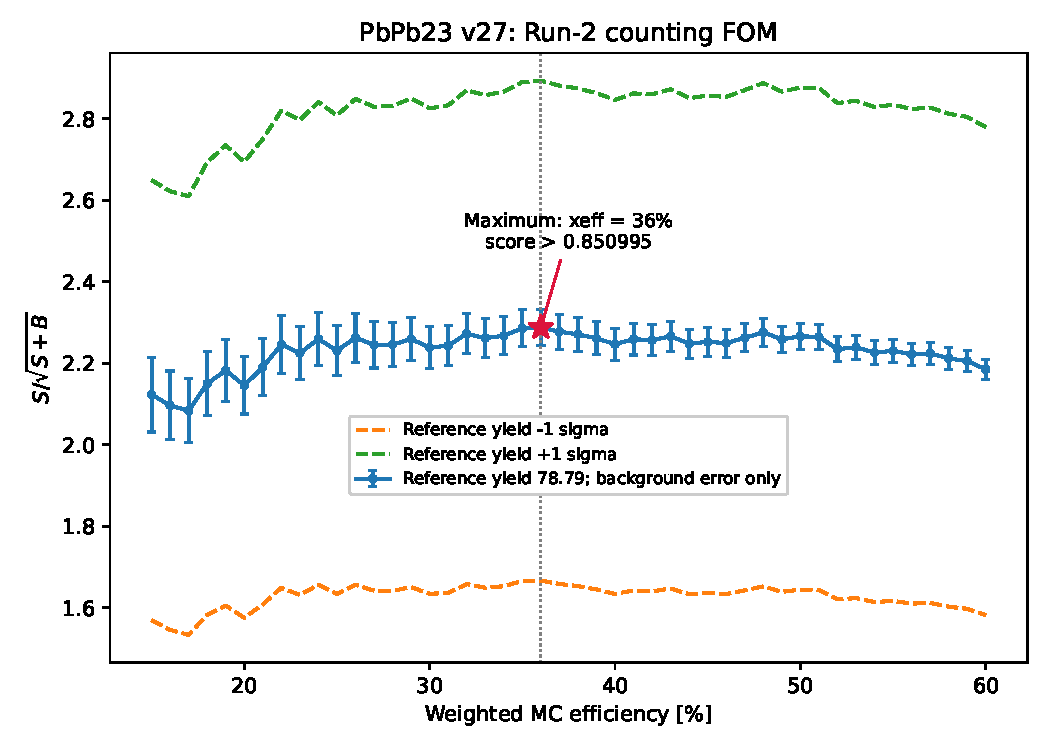
\includegraphics[width=\linewidth,height=0.46\textheight,keepaspectratio]{figures/20260916/fom/fom_xeff.pdf}
    \column{0.49\textwidth}\centering
    {\small\textbf{FOM vs score threshold}}\par
    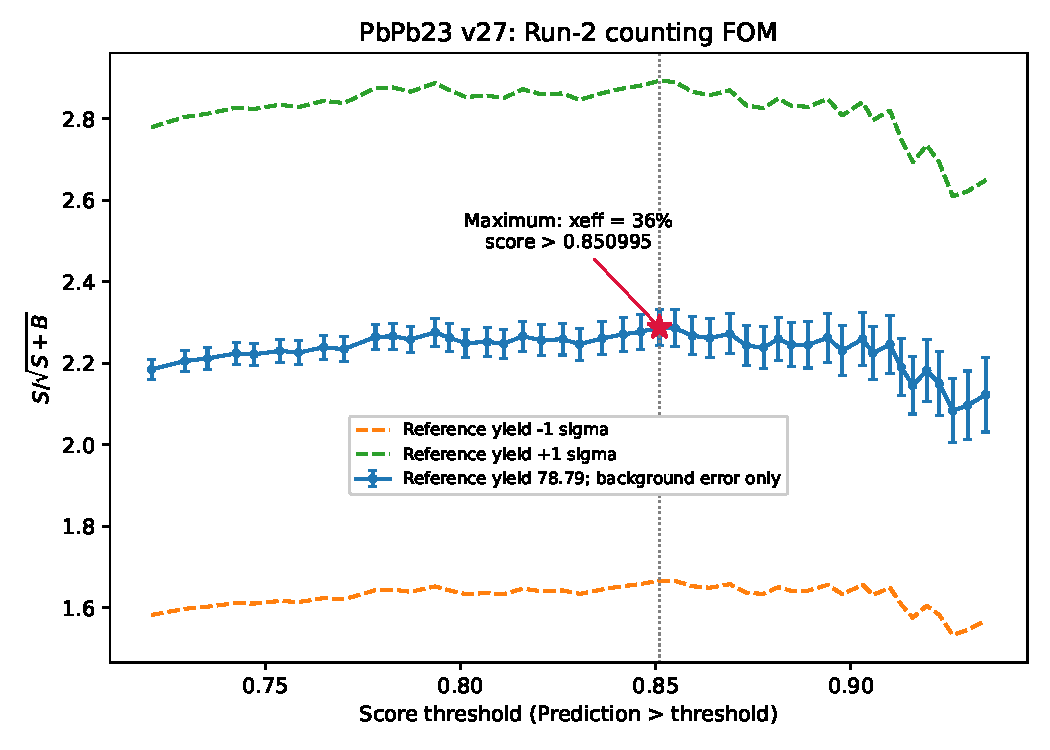
\includegraphics[width=\linewidth,height=0.46\textheight,keepaspectratio]{figures/20260916/fom/fom_score.pdf}
  \end{columns}
  {\small\textbf{Numerical maximum:} $\epsilon_X=36\%$, score $>0.850995$; $S_W=56.66$, $B_W=556.79\pm23.97$.}\par
  {\small FOM: $2.287799$ (36\%) vs $2.266093$ (50\%); improvement $0.958\%$.}\par
  {\small Broad plateau: 35\% gives $2.285971$; $N_{\rm ref}\pm1\sigma$ curves both peak at 36\%.}\par
  \vspace{0.35em}
  \caution{Error bars: background statistics only. Dashed curves: reference-yield variations, not confidence bands.}
  \caution{The 36\% point was frozen before the new DATA fit; FOM is a counting proxy, not significance.}
\end{frame}

\begin{frame}[label=p13_20260916]{Backup: configuration 5 --- fit at the FOM maximum}
  \relax
  {\small Frozen point: $\epsilon_X=36\%$, score $>0.850995$; two-peak fit over $3.62$--$4.00$ GeV.}\par
  \begin{columns}[T]
    \column{0.52\textwidth}\centering
    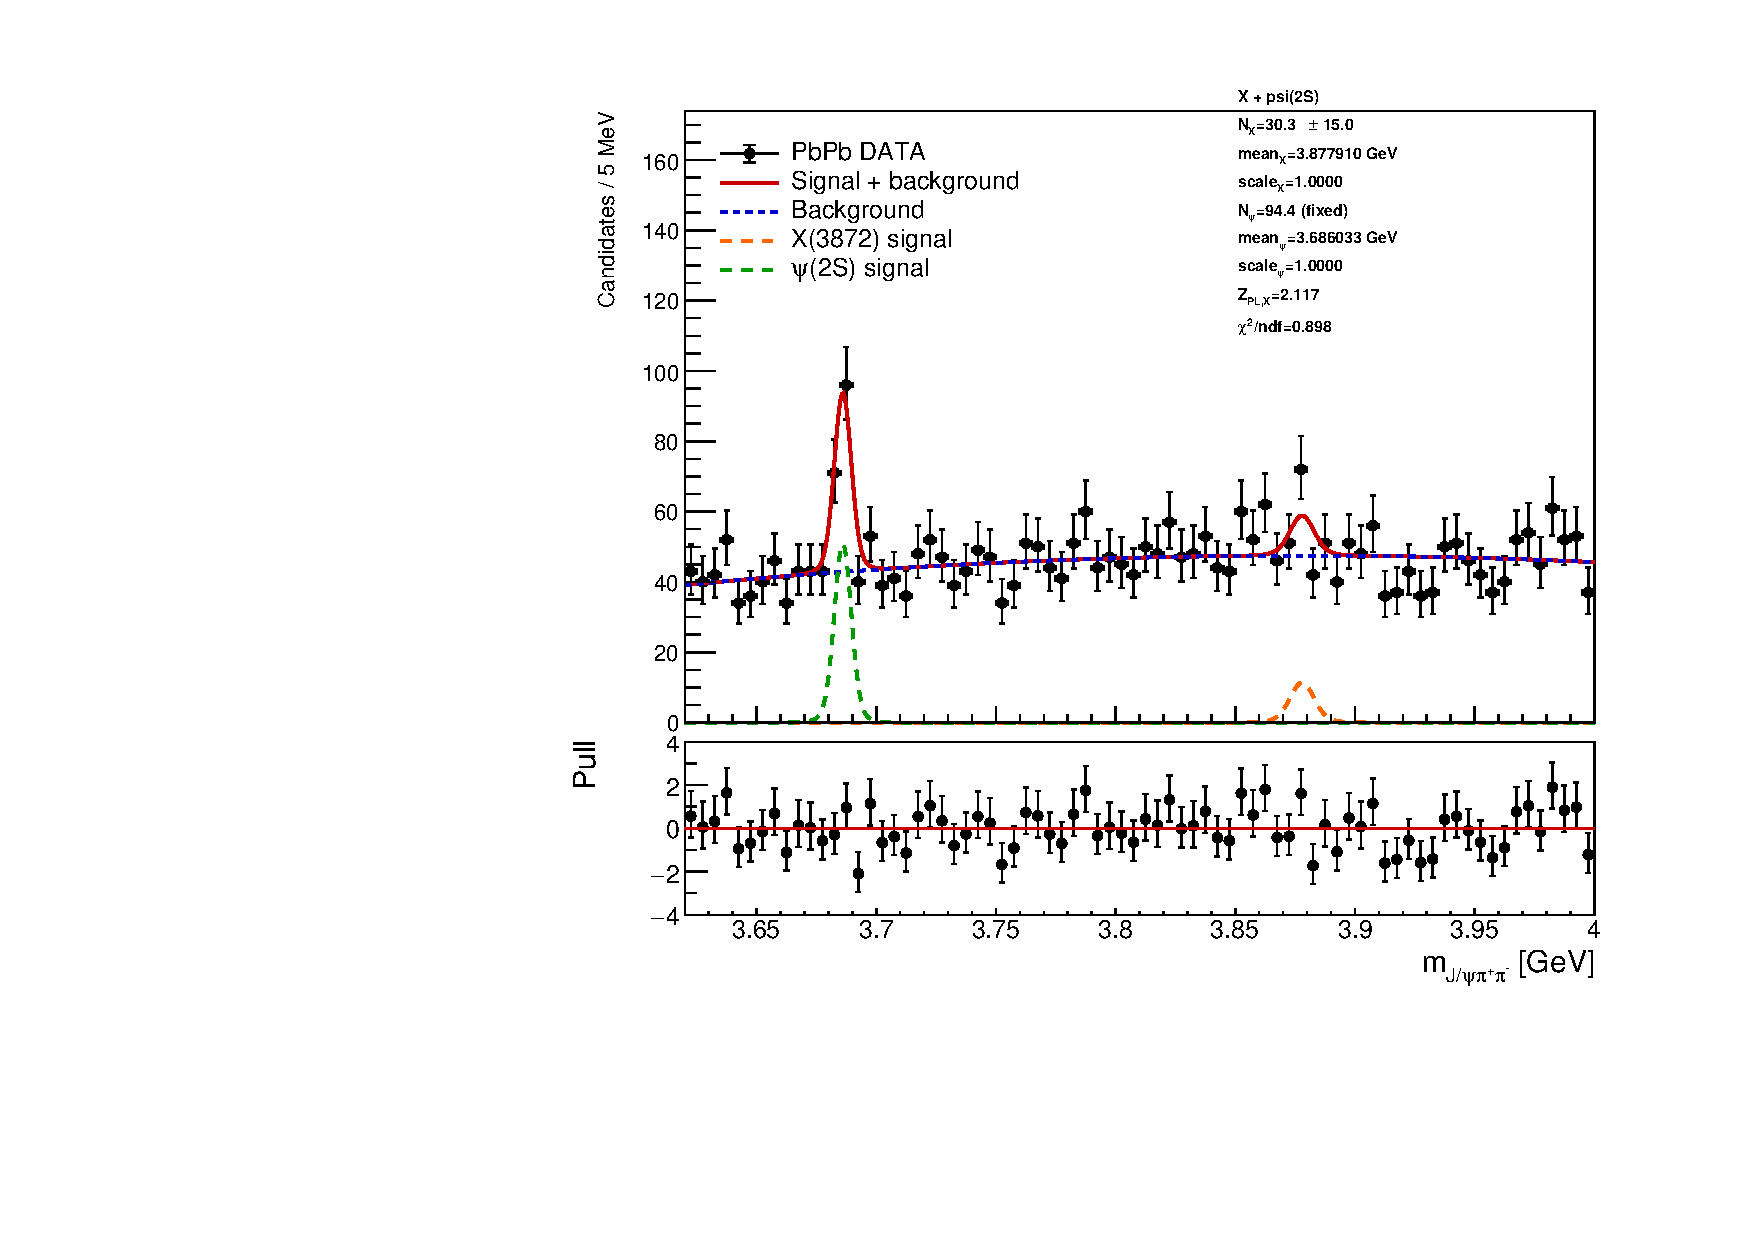
\includegraphics[width=\linewidth,height=0.54\textheight,keepaspectratio]{figures/20260916/fom/xeff36_conditional_fit.pdf}
    \column{0.45\textwidth}\small
    \textbf{36\% fit parameters}\par\vspace{0.3em}
    $\mu_X=3877.91$ MeV (fixed).\par
    $N_\psi=94.35$, $\mu_\psi=3686.03$ MeV (fixed).\par
    \vspace{0.3em}
    Means, $N_\psi$ and background shape fixed\par
    from the first fit; both MC scales fixed to 1.\par
    \vspace{0.5em}
    \begin{tabular}{@{}lcc@{}}
      \toprule
       & 36\% & 50\% reference\\
      \midrule
      FOM & 2.288 & 2.266\\
      $N_X$ & $30.33\pm15.00$ & $78.88\pm21.76$\\
      Significance & 2.117 & 3.873\\
      \bottomrule
    \end{tabular}
  \end{columns}
  \vspace{0.4em}
  {\small\textbf{Higher FOM did not increase the observed significance in this DATA sample.}}\par
  \caution{Broad FOM plateau; no final working point selected.}
\end{frame}


% Optional preview injection; not part of the accepted main deck.
\ifdefined\previewpart
  \input{\previewpart}
\fi

\end{document}
